\chapter{Task 2}
\begin{parlist}
   \item One could use the "Command" design pattern for our project, because commands are sent to the database and they can fail or take too long. It would be useful to save them as objects so that you can undo the changes of the commands to the database if the command is aborted or fails. The "Command" design pattern solves the problem of treating activities/commands like data by wrapping the activities/commands in objects with a consistent interface. And this also allows to undo these commands because the different command objects can also store the data that is modified to be restored when needed.

\item The "Command" pattern Source: Lecture
  \begin{center}
   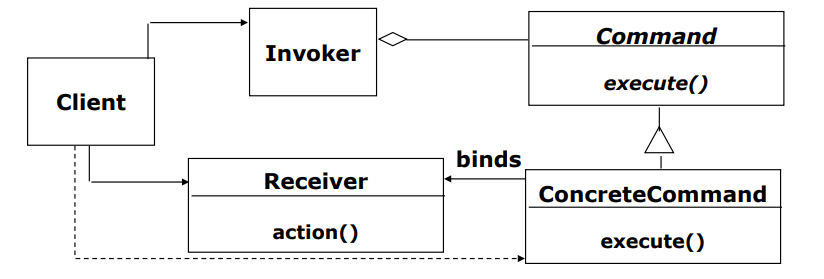
\includegraphics[width=\textwidth]{Immagini/b}
  \end{center}
   \item The "Command" Pattern Applied
     \begin{center}
   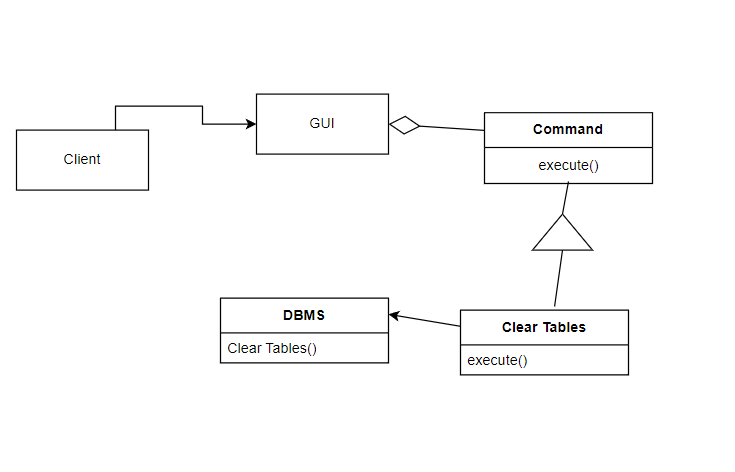
\includegraphics[width=0.9\textwidth]{Immagini/a}
  \end{center}
   \item Pseudo-code for the design pattern: 
\begin{lstlisting}[language=java, frame=trBL]
class Gui{
	Command  clear_command; 
	void Init(){
		clear_command = new ClearTables()
	}
	void OnClickClearTable(){
		clear_command.execute()
	}
}
Interface Command{
	void exectue()
}
class table{
	int id;
	char data[1000];
}
class DBMS{
	void cleartables(List<table>){...}
	List< table> getalltables(){...}
}
class cleartables implements Command{
	List<tables> old_tables;
	@override
	execute(){
		old_tables = DBMS.getalltabels()
		DBMS.cleartables(DBMS.getalltabels())
	}
}
\end{lstlisting}
\end{parlist}
